%%%%%%%%%%%%%%%%%%%%%%%%%%%%%%%%%%%%
% This is the template for submission to ISCA 2019
% The cls file is a modified from  'sig-alternate.cls'
%%%%%%%%%%%%%%%%%%%%%%%%%%%%%%%%%%%%

\documentclass{sig-alternate} 
\usepackage{mathptmx} % This is Times font

\newcommand{\ignore}[1]{}
\usepackage{fancyhdr}
\usepackage[normalem]{ulem}
\usepackage[hyphens]{url}
\usepackage{microtype}
\usepackage{graphicx}
% Always include hyperref last
\usepackage[bookmarks=true,breaklinks=true,letterpaper=true,colorlinks,linkcolor=black,citecolor=blue,urlcolor=black]{hyperref}

% Ensure letter paper
\pdfpagewidth=8.5in
\pdfpageheight=11in


%%%%%%%%%%%---SETME-----%%%%%%%%%%%%%
\newcommand{\iscasubmissionnumber}{NaN}
%%%%%%%%%%%%%%%%%%%%%%%%%%%%%%%%%%%%

\fancypagestyle{firstpage}{
  \fancyhf{}
\renewcommand{\headrulewidth}{0pt}
  \fancyhead[C]{\normalsize{ISCA 2019 Submission
      \textbf{\#\iscasubmissionnumber} \\ Confidential Draft: DO NOT DISTRIBUTE}} 
  \fancyfoot[C]{\thepage}
}  

\pagenumbering{arabic}

%%%%%%%%%%%---SETME-----%%%%%%%%%%%%%
\title{ A Survey of Programming Interface For Persistent Memory} 
\author{}
%%%%%%%%%%%%%%%%%%%%%%%%%%%%%%%%%%%%

\begin{document}
\maketitle
\thispagestyle{firstpage}
\pagestyle{plain}

\begin{abstract}
Non volatile memory provides great advantage but also challenge compared to conventional memory technologies. In this survey we investigate the challenge of persistent programming models and their interface design. We classify and analyze the common errors in persistent memory applications. We believe this survey will motivate more future research in the field for persistent memory software and testing framework.
This survey 

\end{abstract}

\section{Introduction}


STT-RAM \cite{4242474} \cite{6557176}, \cite{Moraru:2013:CDS:2524211.2524216} , and ReRAM \cite{5607274} technologies introduces a new \textit{persistent memory} concept in the memory and storage stack. Persistent memory allows fast byte-addressable access like main memory, and also inherits the data persistence from the storage hardware like disk. Blurring the boundary between DRAM and storage, persistent memory saves the users’ work for (de)serialization and also the overhead in traditional data storage. That’s why persistent memory is also called storage class memory (SCM).

The non-volatility property of persistent memory makes the traditional applications like database, programming language run-time and file system are no longer suitable for persistent memory. First, PM applications store data directly in persistence region in addition to accessing data through more traditional block-based filesystem and database interfaces, we also need to consider the dependency and performance between operating system, hardware with the PM application to achieve better performance and better management, like in heterogeneous memory systems.

	Second, PM applications have to be crash consistent. Volatile programming don’t have issues like that, in PM applications, programmers have to carefully reason about what struct to store and their order. At low level, these properties are ensured by two primitives, (1) clflush, literally cache line flush back, to explicitly write data back fro m the processor cache to the persistent memory. (2) fense, enforcing ordering between writes to dependent structures [15]. The set of writes between ordering points constitute an epoch \cite{Condit:2009:BIT:1629575.1629589} \cite{Pelley:2014:MP:2665671.2665712} and can reach PM in any order, and between epochs, the store operations are strictly ordered. 

Software can implement persistent transactions with ACID semantics using the ordering guarantees of epochs. But there are still issues with raw transactions mechanism as real world data structures are highly related, we may need highly crash consistency model to ensure this.

\vspace{1ex}Contributions: In this paper, we present a survey that:

\begin{itemize}
\item investigates the mainstream persistent memory applications and their interface(APIs)
\item investigates the theory foundation for crash consistency and their application in software design.
\item propose an application level hierarchy to classify different sources of bugs, which could be combined to testing framework by stacked checkers
\item describe the bugs in these class and analyze their relationship with interface design and programming habits

\end{itemize}

\section{An Overview of PM programming models and APIs}

What is a better interface? To guarantee consistency and durability, raw non-volatile structures must meet a bunch of challenges which do not appear in volatile memory. Like dangling pointers, which will not be retrieved after reboot, will be serious issue for persistent memory, multiple free()s, memory leaks and locking errors. Moreover, there are many implicit programming errors, like pointers from non-volatile data structures into volatile memory are unsafe, as when the program crashes, the non-volatile pointer still exists, but it becomes a null pointer. Trusting the users to reason about all and write robust and safe code is dangerous and highly inefficient. So a good interface must be: 



\begin{itemize}
\item Easy to understand, users can draw experiences from former volatile memory programming
\item Expose less internal details about PM models, then the users don’t need to reason much about the hardware.
\item Less programming invariants or rules, that programming will be less error-prone.
\end{itemize}

The naive approach is exposing NVMs as raw storage, which is mapping PM into virtual address space and managing non-volatile memory using volatile memory model. Although this method is easy to understand and familiar to volatile memory programmers, it is error-prone and hard to work with. NV-heaps \cite{Coburn:2011:NMP:1961296.1950380} provides a persistent object system for providing transactional semantics and a robust persistence model. To ensure crash consistency, the system provide safety mechanism in garbage collection, pointer safety and easy-to transactions, while the performance is close to raw NVM. Moreover, the NV-heaps is built on existing file systems and tools, which require less modification to the operating system thus very user-friendly.

	Mnemosyne \cite {Volos:2011:MLP:2248487.1950379}, an interface for persistent programming, provides another way to integrate with the traditional software stack. The purpose of Mnemosyne is to reduce the store overhead in persistence memory. In Mnemosyne, users write data to storage directly rather than writing the pages back through filesystem. The ordering of writes is controlled by software using PM primitives. The system ensure consistency through a lightweight transaction mechanism, which has more flexible than NV-heaps.

	When using low-level primitives, omission of even a single flush, fense operation can result in errors. As undo/redo logs are very common operations in persistent memory, the \textit{transaction} concept is proposed to work as a more organized way to ensure crash consistency and avoid writing the same functional code over and over again in low-level library. Marathe et al. notices the transaction implementation is highly related to the specific run-time system and lack optimization \cite{DBLP:journals/corr/abs-1804-00701}.The paper presents three basic transaction run time and a memory management algorithm to optimize the number of persistent barrier, which is heavy overhead in run time.

	As for concurrency, Kolli et al. proposes a relaxed crash consistency model to optimize the transactions in multi-threading \cite{Kolli:2016:HTP:2954679.2872381}. The system makes use of a deferred commit transactions to minimize persist dependencies and achieve high performance. The work also presents a performance analysis framework for transactions.

	When integrated with programming language and its object system, the interaction of persistent memory with object-oriented programming (OOP) need to be considered. OOP complicates the allocations and deallocation behavior, makes the data access become encapsulated and segmented. The inheritance and composition makes the data store implicit, either in non-volatile and volatile memory. Ren et al. design a new dichotomy design pattern to separate allocation and access \cite{Ren:2017:PNM:3124680.3124729}. In addition, a programming language with managed run-time system makes the problem even harder. This additional layer of abstraction brought the JAVA virtual machine complicate the persistence management. Wu et al. presents Espresso \cite {Wu:2018:EBJ:3173162.3173201}, a general persistent heap to achieve object persistence. A new abstraction called Persistent Java Object is also designed to provide an easy-to-use programming model, while being compatible to existing data structures in Java programs.

	Combining hardware design with the software also attracts many researchers. Narayanan et al. \cite{Narayanan:2012:WP:2248487.2151018} works on a full non-volatile memory system. Their approach is to flush the CPU registers and cache data to the persistent memory only on a failure by hardware. On the reboot, the OS and application are working as a whole system log and then are recovered. But the systems lack extensibility and scalability. 

	Similarly, Zhao et al. takes a milder approach by designing a non-volatile last level cache and main memory to construct a persistent memory hierarchy. In this system, the newly updated data is persisted in cache line and the old data is stored in main memory. The system allows persistent in-place updates without logging. 

	There are also testing framework that aimed at rectifying users’ programming error by testing. The NVL-C \cite{Denny:2016:NSA:2907294.2907303} proposes a programming model, its prototype and a novel static analyses and transformations that test the program at compile time. But static analysis is weak in dynamically allocated structures, so dynamic analysis tools like Yat \cite{Lantz2014YatAV} appears. Yat took an exhaustive searching approach to find every possible execution in run-time and test the memory snapshots with the checkers. Liu et al. proposes PMTest \cite{PMtest01}, a test framework that provides both low-level and high-level checkers to test a wide range of persistent memory. It is easily integrated with other software stacks and requires writing little glue code to reuse the primitives of the test framework.



\begin{figure}
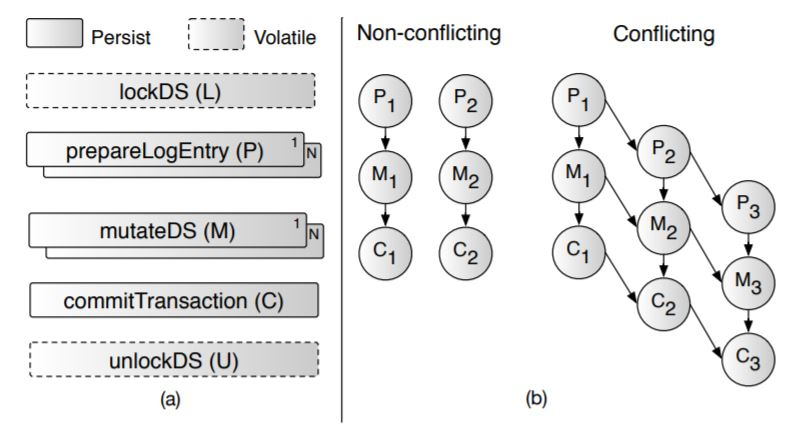
\includegraphics[width=8cm]{pmmodel}
\textbf{Figure 1.} (a) Steps in an undo transaction (b) Persist dependencies in a transaction sequence 
\end{figure}

\section{Crash Consistency Model}

programming in persistent memory introduces the basic idea of crash consistency, which is durability and ordering. Simply write to persist memory don't literally persist them. To solve the program, the clwb operation is provided for durability to make sure that the cache line is written back and thus we can ensure the data to be persisted. Enforcing the ordering is another fundamental function for crash consistency software (CCS). An ordering guarantee from PM system is the fense operation. For example, the common undo log requires the log to be persist before updating the transaction. These strict ordering relationship requires a semantic order constraints for CCS.

	But considering multiprocessors, programming becomes more tricky. Compared to traditional memory model, NVRAM requires a memory model because of the crash consistency. Moreover, in performance for example, NVRAM technologies exhibit asymmetric read and write latencies. It is a completely different scenario for application design and programming primitives. Models about memory consistency has been explored very completely \cite{546611}. It allows programmer to reason about the visible order of loads and stores among threads. Sequential Consistency(SC), requires that all loads and stores occur as some interleaving of program orders of each thread, often requires delays.
	To achieve better performance, relaxed consistency models explicitly allow certain memory operation to reorder. In a thread's perspective, the ordering from other threads are therefore different. But in memory persistency, the recovery mechanisms define specific orders on persists. Like in figure2, the store a must be before store b as the semantics requirement. But if the former memory model reorders them, the persistent consistency is failed. The paper \cite{Pelley:2014:MP:2665671.2665712} regard failure as a recovery observer that atomically reads all of persistent memory at the moment of failure. Ordering constraints thus become ordering constraints on memory and persistent operations as viewed from the recovery observer. With this abstraction, we can borrow some tools from meory consistency -- any two stores to the persistent memory may apply an ordering constraints, which is defined by the oberser. However, these consistency model in Figure 1 can be further relaxed in \cite{Kolli:2016:HTP:2954679.2872381}, which makes the multiprocessor memory application design more flexible, but also more error-prone. 
	In this way, we define a new memory order by our model. The program execution basically defines an order. We separate the memory order of volatile memory and persistent memory and look at our implementation in \cite{Pelley:2014:MP:2665671.2665712}. 

\begin{figure}[b]
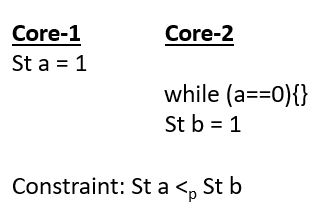
\includegraphics[width=4cm]{mt2}
\textbf{Figure 2.} a,b=0 at initial 
\end{figure}

\subsection{Strict Persistency}  

Our first persistency model is strict persistency. Strict persistency is very easy to implement and simply greatly reasoning about persistent ordering by coupling persist dependences to the memory consistency model. 
\textbf{Definition} Strict persistency persist order observes all partial order implied by volatile memory order. Therefore, the program order is the persists order. We can make sure safety by these strict model.
\textbf{Implementation} An obvious implementation is to stall the next operation util the afore-executed operation is done. Conventional prediction mechanisms may allow loads to speculatively reorder. Buffered strict persistency can be utilized tby serializing persists to a single ordered queue.

\subsection{Relaxed Persistency}

Strict persistency is safe but lack flexibility. Therefore, a relaxed persistency model is proposed to decouple memory consistency and persistency model, as they are actually separate and have gaps to achieve better performance.
	Relaxed persistency loosens persist ordering constraints by application-defined barrier to enforce the visibility of memory operation ordering with respect to other processors.Using the language of ordering constraints in \cite{Kolli:2016:HTP:2954679.2872381}:

\begin{itemize}
\item $L^{i}_a$ : A load from thread i to address a
\item $S^{i}_a$ : A store from thread i to address a
\item $M^{i}_a$ : A memory operation load/store from thread i to address a
\item A $\leq_v$ B: A occurs no later than B in volatile memory order
\item A $\leq_p$ B: A occurs no later than B in non-volatile memory order
\end{itemize}

We describe two relaxed persistency models.

\textbf{Epoch persistency} The epoch persistency model introduces the persist barrier. We denote the persist barriers issued by thread i as $PB^{i}$
Under epoch persistency, any two memory accesses on the same thread that are separated by a persist barrier in volatile memory are ordered in persistent memory:
\\
$M^{i}_a$ $\leq_v$ $PB^{i}_a$ $\leq_v$ $M^{i}_b$   ->  $M^{i}_a$ $\leq_p$ $M^{i}_b$ 
\\

\textbf{Strand Persistency} Strand persistency divides program execution into strands. Those strands are logically independent segments that live in the same thread. New Strands event from thread i are denoted as $NV^{i}$. The new thread event clears all prior PMO constraints from prior instructions.Memory access within a strand are ordered using epoch persistency. 

But in strand consistency, two memory accesses on the same thread separated by a barrier are ordered in persistent memory only if there is no intervening strand barrier.

\section{Taxonomy Of API}

There are now so many interfaces and their own coding rules, mechanisms and invariants. A review of different API is the first step to understand the programming errors. We summarize the existing persistent programming interface and classify them by control granularity. Fine-grained control is more difficult and requires the user to understand more about persistent memory, but can give experienced programmers more freedom in controlling the details and thus achieve high performance. Coarse-grained control is often for high-level application to write fast code and reduce the possibility of errors, but it is encapsulated as high level primitives which users have no control over internal operations.
\subsection{Low-Level API}

The low-level primitives fully expose the requirement of persistent memory to programmers, thus it is the most difficult API. Programmers have to carefully write every NVM access and reason about their orders. Like the Intel PMDK library, provides a libpmem library with a wrapper pmem\_ersist() that is CLWB and FENSE. The libpmem also provides basic cache line flush back and persist barriers. Ren et al. uses a independent syntax to summarize this: \_\_nv(variables ...){ statements; ...}, which means to persist these variables using these primitives \cite{Ren:2017:PNM:3124680.3124729}. 
\subsection{Transaction API}
To save the burden to write naive undo/redo code in every NVM access, a compiler can help to do the work to automatically convert users' connotation to the store inside a transaction. Mnemosyne\cite{Volos:2011:MLP:2248487.1950379} leverages this approach. In transaction API, a programming only need to specify a block of code and use the transaction macro, then every memory access will be taken care of by the transaction run-time. If we follow the low-level syntax, a transaction is like a \_\_nv{statements;..}, which don't need to specify the exact variables. Basically, a transaction is considered a atomics operation that could roll back/recover the update when crash happens.


\subsection{Object-Level API}

The low-level primitives and transactions are working as a data access. A system approach is to specify a consistency state, and by making every update persistence consistent, we make the object persistence consistence. The NVL-C \cite{Denny:2016:NSA:2907294.2907303} provides  a prototype programming language, the two constraints are that programmers have to specify non volatile pointers and all referenced objects must be placed in NVMM. The Intel PMDK supports p<> template pointer that take care of both the basic data types and complex user-defined objects. It also provides a smart pointer persistent\_ptr<> that is compatible with modern C++.
	Other specific and specially designed objects protection mechanism like \cite{Venkataraman:2011:CDD:1960475.1960480} \cite{Yang2015NVTreeRC} are internally protected, and the protection is transparent to users who never modify these data structures.
	A more adanced example is to help automate recognizing persistent objects. NVMOVE \cite{Chauhan2016NVMOVEHP}make static analysis about a traditional application and find out which part needs to be persistent if transplanted into PM application.
	
\subsection{Program-Level API}
After object level protection, it's a natural idea to achieve whole program crash consistency protection.  The ThyNVM \cite{7856636} and whole system persistence (WSP) \cite{Narayanan:2012:WP:2248487.2151018} are special architecture designs that can persist the whole space efficiently. WSP flushes volatile CPU states using residual energy on a power outage. ThyNVM frequently generates checkpoints during execution time. The program-level API can directly work with traditional memory code, and transparently guarantees crash consistency of NVMM data.

Based on the different level of programming API, we will describe the common programming bugs, misuse of the programming models.



\section{Taxonomy Of Programming Errors}



\subsection{data structure dependency}

\begin{figure}
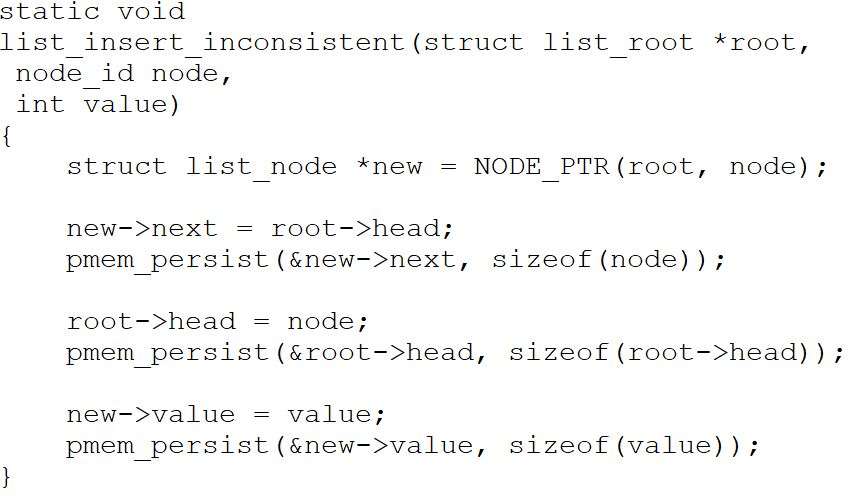
\includegraphics[width=8cm]{error1}
\textbf{Figure 3.} PMDK code to insert a element to a linked list
\end{figure}

In figure2, the code performs the linked list insertion operation. As this is a low-level library, we need to understand the data structures and operations so that we can specify the order explicitly. Because writing undo log for all is not friendly to space usage. The operation is special in that, you need to update the new node and insert it into the linkedlist, or, when you insert the node to the linkedlist, you have to make sure the node is updated. That's the crash consistency for our data structures. This piece of code insert the null node before updating the value. If the system fails before updating, there will be error with the persisted linked list.

	This kind of bugs have something to do with data dependency. In programming, our data often have their own dependency, that when we modify one of them, we need to consider other data that depends on it. In object-oriented design, we design clear and decoupled interface to avoid data entanglement. But in low-level memory model, the reorder of memory writes break the boundary of our interface. Unexpected failure will happen due to the fact that data dependency require the updating to be atomic, or have a specified order.

	The data dependency is very common in low-level library, as in traditional programming model, we do not predict a crash everywhere in the program and thus we don't pay much attention to the order of writes to ensure a safe update. 

\subsection{OO design dependency}

The class Counter is defined to count the events through its function Increase(). It use an array of integers: counts so that threads can be statically assigned to different integers to avoid contention. We define another TimedCounter class to inherit the Counters.

The timedCounter initialize its timestamp with the initialization time. Each increase adds one count. The design follow the encapsulation of OOP. Moreover, the Timedcounter is allocated in non-volatile memory(line 29) and all accesses are protected (Line17).

The program seems plausible, but there is one implicit bug in it. Timedcounter inherits the pointer counts from Counters, and the object is allocated in NVM. Therefore, access to the pointer should be protected with atomic protection. But when we allocate the Counters in Line 5, the counts are not initialized with safety. So the program is buggy due to a implicit data inheritance. These kinds of bugs are also very hard to find.


\begin{figure}
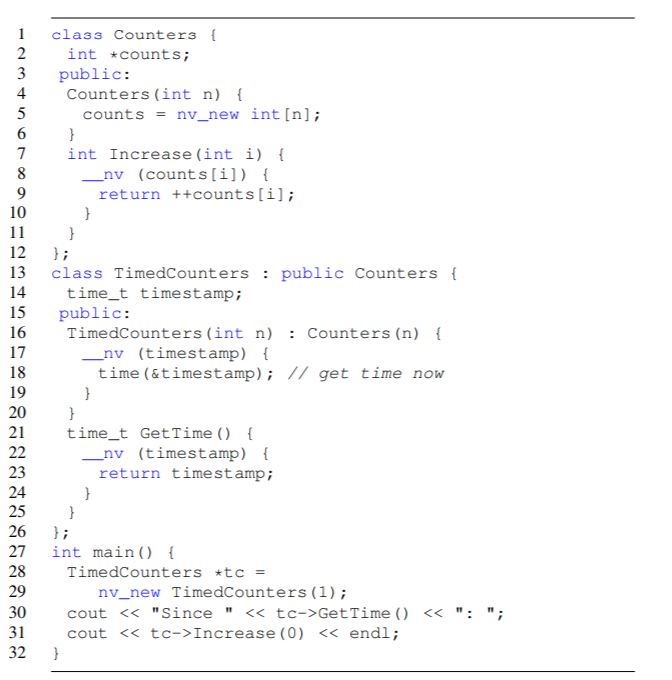
\includegraphics[width=8cm]{error2}
\textbf{Figure 4.} A time counter
\end{figure}


\begin{figure}

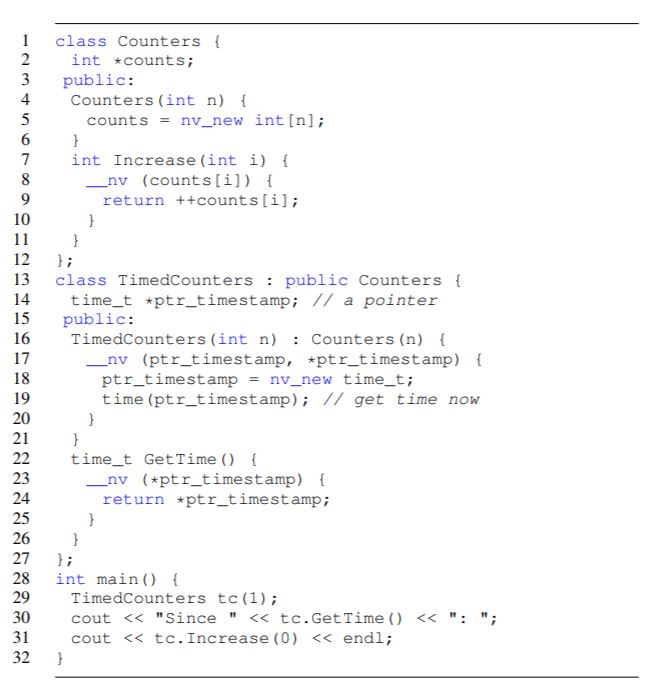
\includegraphics[width=8cm]{error3}
\textbf{Figure 4.} Another time counter
\end{figure}

\textbf{Figure 5.} Another timed counter

Consider another program that allocate the TimedCounter in volatile memory, but the ptr\_timestamp still points to the NVM, while the ptr\_timestamp lives in volatile memory with TimedCounter. But line 16 still protect the pointer, which is unnecessary and affect the performance. In conclusion, mismatch of data placement(in DRAM or NVM) and persistent primitives causes many bugs in persistent programming model.



\subsection{careless mistake}
Last but not least, there are also so many careless mistake made by programmers like forgetting to set transactions, forget the flush back cache line. Especially in complex data structures, these kind of bugs are inevitable even in non-persistent memory programming. Using high-level abstraction could reduce the possibility of such mistakes. 







\section{Conclusion and Future Work}

In this survey, we investigate the PM application and theory for crash consistence. We realize that API designs are really important for users to write safe and high performance code. We classify different granularity of control to the persistent memory. Digging into the bugs and their source, we conclude that:

In the programmers' perspective, API should be designed with less program invariants and be closed to traditional programming. For example, rules like flush back cacheline after writes are extremely error prone. In addition, using a familiar API design like the object protection in \cite{Wu:2018:EBJ:3173162.3173201} is very easy to understand and thus reduce some unexpected mistakes by users.
 
In the software engineering's perspective, API should expose as little internal details as possible. The designer cannot assume that the users to be familiar with persistent memory. The programming rules should be based on a high level concept like a transaction, or even a program-protection system.

There are also another approach that can reduce the programming errors like PMTest \cite{PMtest01}. The paper has already made a unified framework about persistent programming checkers. Future work based on that may be in:
\begin{itemize}
\item We may want to try a learning approach to do automatic bug detection based on static analysis. 
\item Considering the vast amounts of PM application, designing a persistent memory-specific language to unify the different programming models is necessary.
\end{itemize}


%%%%%%% -- PAPER CONTENT ENDS -- %%%%%%%%

%%%%%%%%% -- BIB STYLE AND FILE -- %%%%%%%%
\bibliographystyle{ieeetr}
\bibliography{ref}
%%%%%%%%%%%%%%%%%%%%%%%%%%%%%%%%%%%%

\end{document}
